% ======================================================================
%  From Audio to Beatmap -- the 3-minute cut (10 pages, no overlays)
%  Styled after the app's retro theme: RetroPalette.cs colours, the
%  Audiowide + Press Start 2P fonts, CRT scanlines, the sunset grade.
%
%  Build:  tectonic backend_short.tex      (or: xelatex backend_short.tex)
%          needs XeTeX/LuaTeX for fontspec; fonts are read from fonts/
%  Data:   shared with main.tex -- regenerate with make_data.py
% ======================================================================
\documentclass[aspectratio=169,10pt,t]{beamer}

\usefonttheme{professionalfonts}
\usepackage{fontspec}
\usepackage{amsmath,amssymb}
\usepackage{colortbl}
\usepackage{fancyvrb}
\usepackage{tikz}
\usepackage{pgfplots}
\pgfplotsset{compat=1.18}
\usetikzlibrary{arrows.meta,positioning,calc,decorations.pathreplacing,shadings}
\usepgfplotslibrary{fillbetween}

\input{data/stats.tex}

% ---------------------------------------------------------------- fonts
% the same two faces the app's RetroText renders with. Audiowide has a very
% tall x-height, so it is scaled down to sit at the size of a normal face.
\setsansfont{Audiowide-Regular.ttf}[Path=fonts/,Scale=0.86]
\newfontfamily\pixel{PressStart2P-Regular.ttf}[Path=fonts/]
\newcommand{\px}[1][6]{\pixel\fontsize{#1}{\numexpr#1*2\relax}\selectfont}

% ---------------------------------------------------------------- colours
% straight from frontend/OsuClient.Game/Graphics/RetroPalette.cs
\definecolor{void}{HTML}{0E091C}
\definecolor{panel}{HTML}{170E2C}
\definecolor{inset}{HTML}{0A0614}
\definecolor{magenta}{HTML}{FF2E87}
\definecolor{cyan}{HTML}{29E3FF}
\definecolor{violet}{HTML}{B04AFF}
\definecolor{amber}{HTML}{FFB540}
\definecolor{mint}{HTML}{3DF29C}
\definecolor{bandlow}{HTML}{FF6B52}
\definecolor{bandmid}{HTML}{73F2BF}
\definecolor{bandhigh}{HTML}{99BFFF}
\definecolor{txt}{HTML}{F7F0E6}
\definecolor{dim}{HTML}{B3A8C7}
\definecolor{gradetop}{HTML}{5C1773}
\definecolor{gradebot}{HTML}{F24D59}

% ---------------------------------------------------------------- theme
\setbeamercolor{normal text}{fg=txt}
\setbeamercolor{structure}{fg=magenta}
\setbeamercolor{alerted text}{fg=magenta}
\setbeamertemplate{navigation symbols}{}
\setbeamertemplate{itemize item}{\raisebox{0.15ex}{\color{magenta}\px[5]>}}
\setlength{\leftmargini}{1.1em}
\hyphenpenalty=10000
\exhyphenpenalty=10000

% CRT scanlines: one dark row every millimetre, like ScanlineOverlay
\newcommand{\scanlines}{%
  \foreach \y in {0,0.1,...,9.0}
    \draw[black,opacity=0.22,line width=0.3mm] (0,\y) -- (16,\y);}

\setbeamertemplate{background canvas}{%
  
\begin{tikzpicture}
    \useasboundingbox (0,0) rectangle (\paperwidth,\paperheight);
    \fill[void] (0,0) rectangle (\paperwidth,\paperheight);
    % the sunset grade, rising faintly from the bottom edge
    \shade[bottom color=gradetop!60!void,top color=void] (0,0) rectangle (\paperwidth,2.4);
    \scanlines
  \end{tikzpicture}}

% two-digit tape counter
\newcommand{\counter}{\ifnum\insertframenumber<10 0\fi\insertframenumber}

\setbeamertemplate{frametitle}{%
  \vskip0.22cm
  {\px[6]\color{cyan}TRK \counter\ \ \color{dim}\insertframesubtitle}\par\vskip3pt
  {\fontsize{17}{20}\selectfont\color{txt}\insertframetitle}\par\vskip1pt
  
\begin{tikzpicture}
    \shade[left color=magenta,right color=amber] (0,0) rectangle (4.2,0.07);
    \fill[dim!25] (4.2,0.025) rectangle (\textwidth,0.045);
  \end{tikzpicture}\par\vskip2pt}

\setbeamertemplate{footline}{%
  \hspace*{0.5cm}{\px[5]\color{dim!70}FROM AUDIO TO BEATMAP}\hfill
  {\px[5]\color{magenta}\counter\color{dim!70}/\inserttotalframenumber}\hspace*{0.5cm}\vspace*{0.3cm}}

% ---------------------------------------------------------------- blocks
% the one-line takeaway each slide ends on: an LCD readout off the rack
\newcommand{\readout}[1]{%
  \par\vfill\noindent
  \begin{tikzpicture}
    \node[fill=inset,draw=cyan!45,line width=0.5pt,rounded corners=2pt,inner sep=5pt,
          text width=\dimexpr\linewidth-10pt\relax,font=\small,text=txt,anchor=west] (r) at (0,0)
      {{\px[5]\color{magenta}OUT\ \ }#1};
    \fill[magenta] (r.north west) rectangle ($(r.south west)+(0.07,0)$);
  \end{tikzpicture}\par\vspace*{0.05cm}}

% a small pixel-font label
\newcommand{\kicker}[2]{{\px[5]\color{#1}#2}}

% kicker / centred formula / dim note -- no display-math spacing to fight
\newcommand{\formula}[4]{%
  \kicker{#1}{#2}\par\vspace{4pt}
  {\centering\mbox{$\displaystyle #3$}\par}\vspace{4pt}
  {\scriptsize\color{dim}#4\par}}

\tikzset{
  deck/.style={draw=#1,line width=0.9pt,rounded corners=3pt,fill=panel,
               minimum width=2.05cm,minimum height=1.35cm,text width=1.9cm,align=center,
               font=\scriptsize,text=txt},
  chip/.style={fill=inset,draw=dim!50,rounded corners=2pt,inner sep=4pt,
               font=\scriptsize\ttfamily,text=mint,align=center},
  flow/.style={-{Stealth[length=2.2mm]},line width=0.9pt,color=dim!70},
  note/.style={font=\scriptsize,text=dim,align=center},
  % playfield styles read by data/playfield.tex
  pfpath/.style={dashed,line width=0.7pt,color=dim!70},
  pfcursor/.style={pfpath,shorten <=0.5cm,shorten >=0.5cm},
  pfbody/.style={color=cyan!70,line cap=round,line join=round},
  pfbodyedge/.style={color=cyan!18!void,line cap=round,line join=round},
  pfcircle/.style={circle,draw=magenta,line width=1.3pt,fill=void,text=txt,
                   font=\small,inner sep=0pt},
}

\pgfplotsset{
  every axis/.append style={font=\tiny,axis line style={dim!60},tick style={dim!60},
                            tick label style={text=dim,/pgf/number format/assume math mode=true},
                            label style={text=dim,font=\scriptsize},
                            legend style={fill=none,draw=none,text=txt,font=\tiny},
                            legend cell align=left},
  dspaxis/.style={width=\linewidth,xmin=\statWinStart,xmax=\statWinEnd,
                  axis lines=left,xlabel={time (s)}},
  % keep only rows whose column #1 equals #2
  only kind/.style 2 args={x filter/.append code={%
      \edef\tempa{\thisrow{#1}}\edef\tempb{#2}%
      \ifx\tempa\tempb\else\def\pgfmathresult{inf}\fi}},
}

% ======================================================================
\begin{document}

% ---------------------------------------------------------------- 01 title
\begin{frame}[plain]
  
\begin{tikzpicture}[remember picture,overlay,shift={(current page.south west)}]
    \fill[void] (0,0) rectangle (16,9);
    % sky: the grade deepens toward the horizon
    \shade[bottom color=gradetop,top color=void] (0,3.2) rectangle (16,6.6);
    % striped synthwave sun
    \begin{scope}
      \clip (0,3.2) rectangle (16,9);
      \clip (8,3.2) circle (1.95);
      \shade[top color=amber,bottom color=gradebot] (5.9,3.2) rectangle (10.1,5.2);
      \foreach \y/\h in {3.28/0.16,3.62/0.12,3.93/0.09,4.21/0.065,4.46/0.04}
        \fill[gradetop] (5.9,\y) rectangle (10.1,\y+\h);
    \end{scope}
    % ground grid, rushing toward the viewer
    \fill[void] (0,0) rectangle (16,3.2);
    \begin{scope}
      \clip (0,0) rectangle (16,3.2);
      \foreach \x in {-40,-34,...,56}
        \draw[magenta,opacity=0.55,line width=0.5pt] (8,3.2) -- (\x/2,-3);
      \foreach \k in {1,...,9}
        \draw[magenta,opacity=0.55,line width=0.5pt] (0,{3.2-3.2*(\k/9)^2}) -- (16,{3.2-3.2*(\k/9)^2});
    \end{scope}
    \draw[magenta,line width=1.2pt] (0,3.2) -- (16,3.2);
    % neon title: a soft magenta halo under warm off-white
    \foreach \dx/\dy in {-1.2/0,1.2/0,0/-1.2,0/1.2,-0.8/-0.8,0.8/0.8,-0.8/0.8,0.8/-0.8}
      \node[text=magenta,text opacity=0.35,font=\fontsize{34}{38}\selectfont]
        at ($(8,7.45)+(\dx pt,\dy pt)$) {From Audio to Beatmap};
    \node[text=txt,font=\fontsize{34}{38}\selectfont] at (8,7.45) {From Audio to Beatmap};
    \node[text=dim,font=\large] at (8,6.5)
      {how the backend turns any song into a five-difficulty osu!\ map};
    \node[fill=void,fill opacity=0.85,text opacity=1,inner sep=6pt,rounded corners=2pt,
          draw=cyan!40,text=cyan,font={\px[6]}] at (8,0.75)
      {AUDIO > STFT > FLUX > TEMPO > OBJECTS > .OSZ};
    \scanlines
  \end{tikzpicture}
\end{frame}

% ---------------------------------------------------------------- 02 pipeline
\begin{frame}{One song in, five maps out}{THE PIPELINE}
  A beatmap is a list of objects, and each one needs three answers:\par\vspace{0.5em}
  \begin{center}
  
\begin{tikzpicture}[x=1cm,y=1cm]
    \foreach \x/\h/\c/\t in {0/WHEN/cyan/a time in ms,4.7/WHERE/magenta/a spot on the 512 x 384 field,
                             9.4/WHAT/amber/{circle, slider or spinner}}
      \node[fill=panel,draw=\c!60,rounded corners=2pt,minimum width=4.3cm,minimum height=0.85cm,
            align=center,font=\small,text=txt] at (\x,0) {{\px[5]\color{\c}\h}\\[2pt]\t};
  \end{tikzpicture}
  \end{center}
  \vspace{0.6em}
  \resizebox{\linewidth}{!}{%
  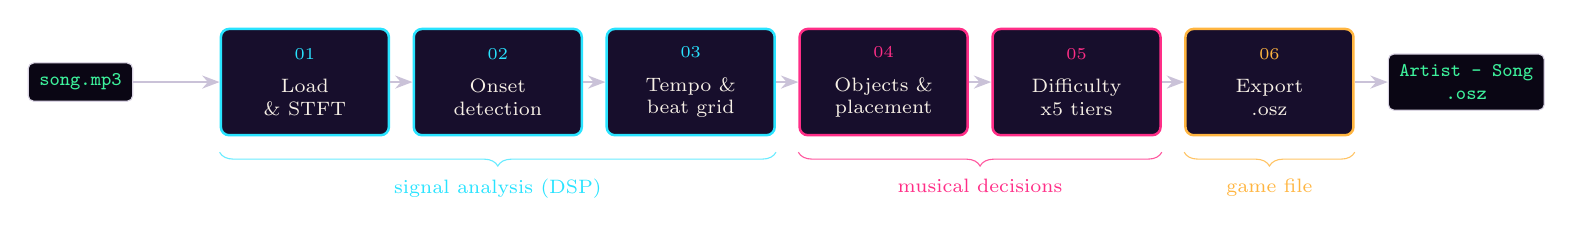
\begin{tikzpicture}[x=1cm,y=1cm]
    \node[chip] (in) at (0,0) {song.mp3};
    \foreach \i/\t/\c in {1/Load\\\& STFT/cyan,2/Onset\\detection/cyan,3/Tempo \&\\beat grid/cyan,
                          4/Objects \&\\placement/magenta,5/Difficulty\\x5 tiers/magenta,6/Export\\.osz/amber}
      \node[deck=\c] (s\i) at (0.4+\i*2.45,0) {{\px[6]\color{\c}0\i}\\[4pt]\t};
    \node[chip] (out) at (17.6,0) {Artist - Song\\.osz};
    \draw[flow] (in) -- (s1);
    \foreach \i [evaluate=\i as \j using int(\i+1)] in {1,...,5} \draw[flow] (s\i) -- (s\j);
    \draw[flow] (s6) -- (out);
    \draw[cyan!70,decorate,decoration={brace,mirror,amplitude=5pt}]
      ($(s1.south west)+(0,-0.2)$) -- ($(s3.south east)+(0,-0.2)$)
      node[midway,below=6pt,note,text=cyan] {signal analysis (DSP)};
    \draw[magenta!80,decorate,decoration={brace,mirror,amplitude=5pt}]
      ($(s4.south west)+(0,-0.2)$) -- ($(s5.south east)+(0,-0.2)$)
      node[midway,below=6pt,note,text=magenta] {musical decisions};
    \draw[amber!80,decorate,decoration={brace,mirror,amplitude=5pt}]
      ($(s6.south west)+(0,-0.2)$) -- ($(s6.south east)+(0,-0.2)$)
      node[midway,below=6pt,note,text=amber] {game file};
  \end{tikzpicture}}
  \readout{One command, {\color{mint}python src/main.py song.mp3}, gives five difficulties from Easy to Expert that the real game imports.}
\end{frame}

% ---------------------------------------------------------------- 03 stft
\begin{frame}{Seeing the song: the mel spectrogram}{STEP 01 / LOAD + STFT}
  \begin{columns}[T]
    \begin{column}{0.56\textwidth}
      \begin{tikzpicture}
        \begin{axis}[at={(0,2.72cm)},anchor=south west,width=6.9cm,height=0.8cm,scale only axis,
                     axis lines=left,xmin=\statWinStart,xmax=\statWinEnd,ymin=-1.05,ymax=1.05,
                     xticklabels=\empty,ytick=\empty,ylabel={audio}]
          \addplot[name path=lo,draw=none] table[col sep=comma,x=t,y=lo]{data/wave.csv};
          \addplot[name path=hi,draw=none] table[col sep=comma,x=t,y=hi]{data/wave.csv};
          \addplot[cyan!80] fill between[of=lo and hi];
        \end{axis}
        \begin{axis}[at={(0,0)},anchor=south west,width=6.9cm,height=2.55cm,scale only axis,
                     axis lines=left,xmin=\statWinStart,xmax=\statWinEnd,ymin=0,ymax=128,
                     enlargelimits=false,xlabel={time (s)},ylabel={mel band},ytick={0,64,128}]
          \addplot graphics[xmin=\statWinStart,xmax=\statWinEnd,ymin=0,ymax=128]{data/melspec.png};
          \draw[cyan,dashed,line width=0.8pt] (axis cs:\statFluxOnsetTime,0) -- (axis cs:\statFluxOnsetTime,128);
        \end{axis}
      \end{tikzpicture}
    \end{column}
    \begin{column}{0.42\textwidth}
      \formula{cyan}{SHORT-TIME FOURIER TRANSFORM}
        {X[m,k]=\textstyle\sum_{n} x[n+mH]\,w[n]\,e^{-j2\pi kn/N}}
        {mono, \statSampleRate\ Hz, peak-normalised}
      \vspace{0.3em}
      \begin{itemize}\footnotesize
        \item \statWinMs\,ms Hann window, \statHopMs\,ms hop: \statFrameRate\ spectra per second
        \item pooled into \textbf{128 mel bands}, fine in the bass and coarse up high, the way hearing works
      \end{itemize}
    \end{column}
  \end{columns}
  \readout{The vertical streaks are broadband \textcolor{cyan}{attacks}. Those are the note starts we want to find.}
\end{frame}

% ---------------------------------------------------------------- 04 onsets
\begin{frame}{Finding every note start}{STEP 02 / ONSET DETECTION}
  \begin{tikzpicture}
    \begin{axis}[dspaxis,height=2.85cm,ymin=0,ymax=1.08,ylabel={flux},
                 legend style={at={(1,1.02)},anchor=south east,legend columns=6}]
      \addplot[dim!70,line width=0.5pt] table[col sep=comma,x=t,y=flux]{data/flux.csv};
      \addlegendentry{spectral flux}
      \addplot[cyan!70,line width=0.9pt] table[col sep=comma,x=t,y=median]{data/flux.csv};
      \addlegendentry{moving median}
      \addplot[magenta,line width=1.2pt] table[col sep=comma,x=t,y=thr]{data/flux.csv};
      \addlegendentry{threshold}
      \addplot[forget plot,scatter,only marks,mark size=1.8pt,scatter src=explicit symbolic,
               scatter/classes={low={mark=*,bandlow},mid={mark=*,bandmid},high={mark=*,bandhigh}}]
        table[col sep=comma,x=t,y=s,meta=band]{data/peaks.csv};
      \addlegendimage{only marks,mark=*,bandlow}\addlegendentry{onset: low}
      \addlegendimage{only marks,mark=*,bandmid}\addlegendentry{mid}
      \addlegendimage{only marks,mark=*,bandhigh}\addlegendentry{high}
    \end{axis}
  \end{tikzpicture}
  \par\vspace{0.2em}
  \begin{columns}[T]
    \begin{column}{0.34\textwidth}
      \formula{cyan}{SPECTRAL FLUX}
        {\mathrm{SF}[m]=\big\|\max(0,\,P_m-P_{m-1})\big\|}
        {energy that appears; fading notes are ignored}
    \end{column}
    \begin{column}{0.34\textwidth}
      \formula{magenta}{ADAPTIVE THRESHOLD}
        {T[m]=\delta+\lambda\cdot\mathrm{median}_{\pm0.5\,\mathrm{s}}\,\mathrm{SF}}
        {tracks quiet verses and loud drops alike}
    \end{column}
    \begin{column}{0.28\textwidth}
      \kicker{amber}{PEAK PICKING}\par\vspace{5pt}
      {\scriptsize local maxima above $T$, at least 50\,ms apart, each tagged with its strongest frequency band\par}
    \end{column}
  \end{columns}
  \readout{\statOnsetsTotal\ onsets in \statDuration\,s, each one carrying its strength and band (low / mid / high).}
\end{frame}

% ---------------------------------------------------------------- 05 tempo
\begin{frame}{How fast is the music?}{STEP 03 / TEMPO}
  \begin{columns}[T]
    \begin{column}{0.55\textwidth}
      \begin{tikzpicture}
        \begin{axis}[width=\linewidth,height=4.2cm,axis lines=left,xmin=50,xmax=210,ymin=0,ymax=1.1,
                     xlabel={tempo (BPM)},legend style={at={(0.5,1.02)},anchor=south,legend columns=3}]
          \addplot[dim!70,mark=*,mark size=0.8pt,line width=0.5pt] table[col sep=comma,x=bpm,y=acf]{data/acf.csv};
          \addlegendentry{autocorrelation $r$}
          \addplot[cyan,dashed,line width=0.9pt] table[col sep=comma,x=bpm,y=prior]{data/acf.csv};
          \addlegendentry{prior $w$}
          \addplot[magenta,line width=1.2pt,mark=*,mark size=1pt] table[col sep=comma,x=bpm,y=weighted]{data/acf.csv};
          \addlegendentry{$r\cdot w$}
          \draw[amber,dashed,line width=0.8pt] (axis cs:\statBPM,0) -- (axis cs:\statBPM,0.82)
            node[above,font=\tiny,text=amber] {\statBPM};
        \end{axis}
      \end{tikzpicture}
    \end{column}
    \begin{column}{0.43\textwidth}
      \formula{cyan}{AUTOCORRELATION (WIENER-KHINCHIN)}
        {r=\mathcal{F}^{-1}\big\{|\mathcal{F}\{e\}|^2\big\}}
        {a beat is a repeating ripple in the flux; $r$ peaks at its period}
      \vspace{0.6em}
      \kicker{magenta}{PRIOR + OCTAVE CHECK}\par\vspace{4pt}
      {\scriptsize\color{dim}a log-normal prior around 120 BPM, then: which pulse train really lands on the hits?\par}
      \vspace{4pt}
      {\scriptsize\arrayrulecolor{dim!50}\renewcommand{\arraystretch}{1.15}
      \begin{tabular}{@{}l r r@{}}
        \kicker{dim}{CANDIDATE} & \kicker{dim}{BPM} & \kicker{dim}{SCORE}\\\hline
        half & \statOctHalfBPM & \statOctHalfScore\\
        \rowcolor{magenta!30!void}
        found & \statOctOneBPM & \statOctOneScore\\
        double & \statOctDoubleBPM & \statOctDoubleScore\\
      \end{tabular}}
    \end{column}
  \end{columns}
  \readout{Autocorrelation finds the period; the prior and octave check keep it off half or double tempo. Result: \textcolor{amber}{\statBPM\ BPM}.}
\end{frame}

% ---------------------------------------------------------------- 06 grid
\begin{frame}{Locking to the beat grid}{STEP 03 / PHASE + SNAP}
  \begin{tikzpicture}
    \begin{axis}[dspaxis,height=2.85cm,ymin=0,ymax=1.12,ylabel={flux},
                 legend style={at={(1,1.02)},anchor=south east,legend columns=4}]
      \addplot[ycomb,dim!25,line width=0.4pt,mark=none] table[col sep=comma,x=t,y expr=1.1]{data/grid.csv};
      \addlegendentry{1/4 grid}
      \addplot[ycomb,magenta,line width=1.1pt,mark=none] table[col sep=comma,x=t,y expr=1.1]{data/beats.csv};
      \addlegendentry{beats}
      \addplot[dim!70,line width=0.5pt] table[col sep=comma,x=t,y=flux]{data/flux.csv};
      \addlegendentry{flux}
      \addplot[only marks,mark=*,mark size=1.6pt,amber] table[col sep=comma,x=t,y=s]{data/peaks.csv};
      \addlegendentry{onsets}
    \end{axis}
  \end{tikzpicture}
  \par\vspace{0.2em}
  \begin{columns}[T]
    \begin{column}{0.48\textwidth}
      \formula{magenta}{PHASE: WHERE IS BEAT ONE?}
        {\varphi^\ast=\arg\max_{\varphi}\ \tfrac1N\textstyle\sum_n e(\varphi+nP)}
        {slide a pulse train across one beat; keep the offset that collects the most energy}
    \end{column}
    \begin{column}{0.48\textwidth}
      \formula{amber}{SNAP: EACH ONSET TO ITS NEAREST SLOT}
        {\hat t=\varphi^\ast+\mathrm{round}\big(\tfrac{t-\varphi^\ast}{P/d}\big)\,\tfrac{P}{d}}
        {removes detector jitter; two onsets in one slot keep the stronger (\statSnapMerged\ merged)}
    \end{column}
  \end{columns}
  \readout{One constant grid (offset \statOffset\,ms, a beat every \statBeatMs\,ms) is what makes a map feel snapped to the music.}
\end{frame}

% ---------------------------------------------------------------- 07 objects
\begin{frame}{Circle, slider or spinner?}{STEP 04 / CLASSIFICATION}
  \begin{columns}[T]
    \begin{column}{0.53\textwidth}
      \begin{tikzpicture}
        \begin{axis}[dspaxis,height=3.2cm,ymin=0,ymax=1.08,ylabel={RMS / peak},unbounded coords=discard,
                     legend style={at={(1,1.02)},anchor=south east,legend columns=4}]
          \addplot[cyan!80,line width=0.7pt] table[col sep=comma,x=t,y=rms]{data/rms.csv};
          \addlegendentry{RMS energy}
          \addplot[ycomb,magenta,line width=0.8pt,mark=*,mark size=1.2pt,only kind={kind}{circle}]
            table[col sep=comma,x=t,y expr=1.0]{data/objects.csv};
          \addlegendentry{circle}
          \addplot[ycomb,mint,line width=1.4pt,mark=square*,mark size=1.6pt,only kind={kind}{slider}]
            table[col sep=comma,x=t,y expr=1.0]{data/objects.csv};
          \addlegendentry{slider}
          \addplot[amber,dashed,line width=0.8pt,domain=\statWinStart:\statWinEnd,samples=2] {0.15};
          \addlegendentry{15\%}
        \end{axis}
      \end{tikzpicture}
      \par\vspace{0.2em}
      {\scriptsize\color{dim}\textcolor{txt}{Sustain ratio $s$}: the share of frames after a hit that stay
      above \textcolor{amber}{15\% of peak}. Near 1, the note rings on; near 0, it decayed.\par}
    \end{column}
    \begin{column}{0.45\textwidth}
      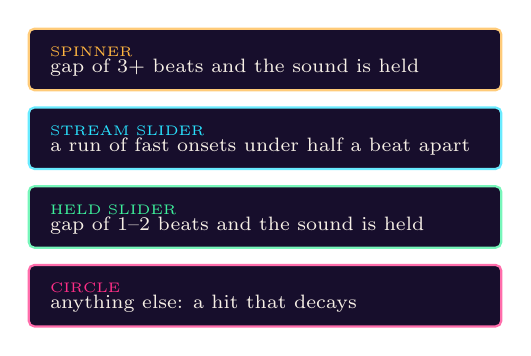
\begin{tikzpicture}[x=1cm,y=1cm]
        \foreach \y/\c/\k/\r in {0/amber/SPINNER/gap of 3+ beats and the sound is held,
                                  -1.0/cyan/STREAM SLIDER/a run of fast onsets under half a beat apart,
                                  -2.0/mint/HELD SLIDER/gap of 1--2 beats and the sound is held,
                                  -3.0/magenta/CIRCLE/anything else: a hit that decays}{
          \node[fill=panel,draw=\c!70,line width=0.8pt,rounded corners=2pt,minimum width=6cm,
                minimum height=0.78cm,anchor=west] at (0,\y) {};
          \node[anchor=north west,text=\c,font={\px[5]}] at (0.16,\y+0.28) {\k};
          \node[anchor=south west,font=\scriptsize,text=txt] at (0.16,\y-0.34) {\r};
        }
      \end{tikzpicture}
      \par\vspace{0.2em}{\scriptsize\color{dim}checked top to bottom; the first rule that fits wins\par}
    \end{column}
  \end{columns}
  \readout{The \emph{shape} of the energy after a hit decides the object: a tap decays, a hold rings on.}
\end{frame}

% ---------------------------------------------------------------- 08 placement
% playfield.tex carries overlay specs <2->..<8>; show only its final state
\begin{frame}<8>{Placing objects like a mapper would}{STEP 04 / PLACEMENT}
  \begin{columns}[T]
    \begin{column}{0.44\textwidth}
      \centering
      \scalebox{0.72}{%
      \begin{tikzpicture}[x=\statPFScale cm,y=-\statPFScale cm]
        \draw[dim!50,fill=panel,rounded corners=2pt] (0,0) rectangle (512,384);
        \draw[dim!20,dashed] (40,40) rectangle (472,344);
        \input{data/playfield.tex}
      \end{tikzpicture}}
      \par\vspace{2pt}{\scriptsize\color{dim}\statTier: \statPFCount\ objects in play order, true scale\par}
    \end{column}
    \begin{column}{0.54\textwidth}
      \formula{cyan}{DISTANCE SNAP}
        {d=D\cdot\sigma\cdot\Delta b}
        {distance grows linearly with the gap $\Delta b$ in beats, in circle diameters $D$;
         $\sigma$ runs from 0.85 (Easy) to 2.10 (Expert)}
      \vspace{0.6em}
      \kicker{magenta}{A VIRTUAL CURSOR WALKS THE MAP}
      \begin{itemize}\scriptsize
        \item \textbf{flow}: small turns over short gaps so streams arc; sharp turns only on jumps
        \item \textbf{never bury}: at least $0.75\,D$ from the previous object
        \item \textbf{stay off slider bodies}: clear the whole drawn curve, not just its ends
      \end{itemize}
    \end{column}
  \end{columns}
  \readout{Mapping conventions become geometry: how far apart two objects are tells the player the rhythm.}
\end{frame}

% ---------------------------------------------------------------- 09 difficulty
\begin{frame}{One analysis, five difficulties}{STEP 05 / DIFFICULTY}
  \begin{columns}[T]
    \begin{column}{0.52\textwidth}
      \vspace{0.3em}
      {\scriptsize\arrayrulecolor{dim!50}\renewcommand{\arraystretch}{1.3}
      \begin{tabular}{@{}l c c c@{}}
        \kicker{dim}{KNOB} & \textcolor{cyan}{Easy} & \textcolor{amber}{Hard} & \textcolor{violet}{Expert}\\\hline
        threshold $\lambda$ / $\delta$ & 2.2 / .08 & 1.5 / .05 & 1.1 / .03\\
        snap grid & 1/1 & 1/4 & 1/4\\
        min spacing (beats) & 2.0 & 0.5 & 0.25\\
        distance $\sigma$ & 0.85 & 1.3 & 2.10\\
        max turn & 40\textdegree & 75\textdegree & 130\textdegree\\
        AR / OD / CS & 4 / 3 / 3.2 & 7.5 / 6 / 4 & 9.3 / 8.5 / 4.2\\
      \end{tabular}}\par\vspace{0.8em}
      {\footnotesize The \textcolor{cyan}{DSP knobs} set how many onsets exist. The
      \textcolor{magenta}{musical knobs} set how many survive and how they move.\par}
    \end{column}
    \begin{column}{0.46\textwidth}
      \begin{tikzpicture}
        \begin{axis}[width=\linewidth,height=4.4cm,ybar,bar width=14pt,axis lines=left,ymin=0,ymax=1200,
                     symbolic x coords={Easy,Normal,Hard,Insane,Expert},xtick={Easy,Normal,Hard,Insane,Expert},
                     enlarge x limits=0.14,ylabel={objects},ytick={0,500,1000},
                     nodes near coords,point meta=y,
                     every node near coord/.append style={font={\px[5]},text=txt,
                       /pgf/number format/assume math mode=true,/pgf/number format/1000 sep={}}]
          \addplot[fill=cyan,draw=none,bar shift=0pt] coordinates {(Easy,\statObjEasy)};
          \addplot[fill=mint,draw=none,bar shift=0pt] coordinates {(Normal,\statObjNormal)};
          \addplot[fill=amber,draw=none,bar shift=0pt] coordinates {(Hard,\statObjHard)};
          \addplot[fill=magenta,draw=none,bar shift=0pt] coordinates {(Insane,\statObjInsane)};
          \addplot[fill=violet,draw=none,bar shift=0pt] coordinates {(Expert,\statObjExpert)};
        \end{axis}
      \end{tikzpicture}
      \par{\centering\scriptsize\color{dim}objects per tier, \SongFile\par}
    \end{column}
  \end{columns}
  \readout{The audio is analysed once and re-read with five presets, so one song becomes a full beatmap set.}
\end{frame}

% ---------------------------------------------------------------- 10 export
\begin{frame}[fragile]{A file the real game accepts}{STEP 06 / EXPORT + TESTING}
  \begin{columns}[T]
    \begin{column}{0.5\textwidth}
      \kicker{mint}{OSU FILE FORMAT V14}\par\vspace{4pt}
      \fvset{fontsize=\fontsize{4.8}{5.6}\selectfont,frame=single,rulecolor=\color{dim!40},
             framesep=1.5mm,formatcom=\color{mint}}
      \VerbatimInput{data/osu_excerpt.txt}
      \vspace{2pt}
      {\scriptsize\color{dim}five .osu files + the audio, zipped into one .osz; an analysis.json keeps
      the onsets, grid and spectrogram for the app to show\par}
    \end{column}
    \begin{column}{0.48\textwidth}
      \kicker{amber}{NO GROUND TRUTH, SO TEST THREE WAYS}
      \begin{itemize}\scriptsize
        \item \textbf{synthetic signals}: click tracks at a known BPM, held tones, fast bursts,
              each with an exact expected answer
        \item \textbf{listening}: a click on every onset and a metronome on every beat;
              drift is obvious by ear
        \item \textbf{play-testing} in osu!lazer; every problem found became an automated test
      \end{itemize}
      \vspace{0.4em}
      \begin{center}
        \tikz\node[chip] {pytest: 256 backend tests};
      \end{center}
    \end{column}
  \end{columns}
  \readout{osu!lazer rejects malformed files, so a clean import doubles as the end-to-end test.}
\end{frame}

\end{document}
